\documentclass[a4paper,12pt,titlepage,oneside]{book}
\linespread{1.2}
\pagestyle{plain}


\usepackage[italian]{babel} 
\usepackage{picture}
\usepackage{hyperref}
\usepackage[Symbol]{upgreek}
\usepackage{amsmath}
\usepackage{wrapfig}
\usepackage{siunitx}
\usepackage{caption}
\usepackage{subcaption}
\usepackage{graphicx}
\usepackage{csquotes}
\usepackage{color}
\usepackage{listings}
\usepackage{xcolor}

\definecolor{codegreen}{rgb}{0,0.6,0}
\definecolor{codegray}{rgb}{0.5,0.5,0.5}
\definecolor{codepurple}{rgb}{0.58,0,0.82}
\definecolor{backcolour}{rgb}{0.95,0.95,0.92}

\lstdefinestyle{mystyle}{
    backgroundcolor=\color{backcolour},   
    commentstyle=\color{codegreen},
    keywordstyle=\color{magenta},
    numberstyle=\tiny\color{codegray},
    stringstyle=\color{codepurple},
    basicstyle=\ttfamily\footnotesize,
    breakatwhitespace=false,         
    breaklines=true,                 
    captionpos=b,                    
    keepspaces=true,                 
    numbers=left,                    
    numbersep=5pt,                  
    showspaces=false,                
    showstringspaces=false,
    showtabs=false,                  
    tabsize=2
}

\lstset{style=mystyle}

\usepackage{pdfpages}
\textheight24cm\topmargin0mm\headheight0mm\headsep6mm\oddsidemargin20pt\evensidemargin30pt

\usepackage[T1]{fontenc}
\usepackage[utf8]{inputenc}
\usepackage{titlesec, blindtext, color}
\definecolor{gray75}{gray}{0.75}
\newcommand{\hsp}{\hspace{20pt}}
\titleformat{\chapter}[hang]{\Huge\bfseries}{\thechapter\hsp\textcolor{gray75}{|}\hsp}{0pt}{\Huge\bfseries}

\usepackage{csquotes}
\usepackage[backend=bibtex]{biblatex}
\bibliography{bibliografia}


\definecolor{dkgreen}{rgb}{0,0.6,0}
\definecolor{gray}{rgb}{0.5,0.5,0.5}
\definecolor{mauve}{rgb}{0.58,0,0.82}

\begin{document}

\begin{titlepage}

\newcommand{\HRule}{\rule{\linewidth}{0.5mm}} % Defines a new command for the horizontal lines, change thickness here

\center % Center everything on the page
 
%----------------------------------------------------------------------------------------
%	HEADING SECTIONS
%----------------------------------------------------------------------------------------

\textsc{\LARGE Università degli studi di Milano-Bicocca}\\[1cm] % Name of your university/college
\textsc{\Large Metodi del Calcolo Scientifico }\\[0.3cm] % Major heading such as course name
\textsc{\large Project 2}\\[0.1cm] % Minor heading such as course title

%----------------------------------------------------------------------------------------
%	TITLE SECTION
%----------------------------------------------------------------------------------------

\HRule \\[0.4cm]
{ \huge \bfseries Compressione di immagini tramite la
DCT}\\[0.4cm] % Title of your document
\HRule \\[1.5cm]
 
%----------------------------------------------------------------------------------------
%	AUTHOR SECTION
%----------------------------------------------------------------------------------------

\large
\emph{Authors:}\\
Capra Riccardo - 808227 \\ % Your name
Curnis Giovanni - 807424 \\[1cm]

% If you don't want a supervisor, uncomment the two lines below and remove the section above
%\Large \emph{Author:}\\
%John \textsc{Smith}\\[3cm] % Your name

%----------------------------------------------------------------------------------------
%	DATE SECTION
%----------------------------------------------------------------------------------------

%{\large \today}\\[1cm] % Date, change the \today to a set date if you want to be precise

%----------------------------------------------------------------------------------------
%	LOGO SECTION
%----------------------------------------------------------------------------------------


\includegraphics[scale = 2.5]{src/image/unimib-logo.pdf}\\[1cm] % Include a department/university logo - this will require the graphicx package
 
%----------------------------------------------------------------------------------------

\vfill % Fill the rest of the page with whitespace

\end{titlepage}

\tableofcontents

\chapter{Introduzione}
Questo progetto è diviso in due fasi: della prima fase è implementare un algoritmo di $DCT_2$ in ambiente Open Source e confrontare questa implementazione con quella di una libreria ottimizzata, scopo della seconda fase è creare un interfaccia che consenta di comprimere immagini in toni di grigio per immagini in formato BMP.

\chapter{Cenni teorici}

Per codificare una immagine in scala di grigi o a colori l'operazione che viene effettuata la maggior parte delle volte è quella della trasformata che consente di rappresentare i pixel, normalmente rappresentati da una matrice contenete i valori di luminosità di ogni pixel, in una rappresentazione tramite frequenze. In questo tipo di rappresentazione le onde a bassa frequenza rendono conto dell'andamento generale della luminosità dell'immagine, mentre quelle ad alta frequenza codificano i dettagli e il disturbo introdotto dall'elettronica dei dispositivi di acquisizione.

Normalmente le immagini fotografiche hanno un andamento continuo e quindi la rappresentazione nel dominio delle frequenze  è spesso costituita da una matrice quadrata di valori, dei quali solo quelli corrispondenti alle basse frequenze sono significativi e si trovano nell'angolo in alto a sinistra mentre le frequenze alte hanno una rilevanza minore.

Attenuare ulteriormente le componenti meno significative è possibile, basta dividere ogni coefficiente della matrice trasformata per un certo valore specificato in una tabella, così facendo la matrice risultante conterrà numerosi valori nulli. Questa operazione però causa una grande perdita di qualità ed è nota come quantizzazione e viene usata per ottenere una elevata compressione dell'immagine.

\section{$DCT_2$}
I gruppi di standardizzazione JPEG e MPEG utilizzano la \textbf{Trasformata Discreta del Coseno (DCT)} che essendo capace di rivelare le variazioni di informazione tra un’area e quella contigua trascurando le ripetizioni provvede alla compressione spaziale. Inoltre, essa rappresenta un ottimo compromesso complessità-prestazioni.

Tuttavia la complessità dell'algoritmo DCT cresce molto rapidamente al crescere delle dimensioni dell'immagine e per questa ragione la DCT viene applicata su blocchi più piccoli, ad esempio di 8x8 \textit{px} nei quali viene scomposta.

I numeri contenuti in questi blocchi 8x8 vengono detti \textbf{coefficienti DCT} e descrivono il contenuto delle frequenze sia alte che basse in quel blocco. In teoria questa trasformata dovrebbe essere fedele ma le operazioni in virgola mobile coinvolte e le varie operazioni inducono degli errori di rappresentazione e causano delle perdite di informazione.

Una conseguenza vantaggiosa della DCT è che i valori significativi saranno trasportati in alto a sinistra.

Questo ragionamento è facilmente applicabile anche a più dimensioni. Prendendo un considerazione un array il cui indice è bidimensionale otterremo la seguente formula:
\begin{equation}
    c_{kl} = \alpha_{Kl} \sum^{N-1}_{i=0} \sum^{M-1}_{j=0} f_{ij} \cos ( k \pi \frac{2i + 1}{2N} ) \cos (l \pi \frac{2j + 1}{2M})
\end{equation}

\begin{itemize}
  \item The individual entries are indicated with a black dot, a so-called bullet.
  \item The text in the entries may be of any length.
\end{itemize}


\section{Matrice definita positiva}
In matematica, e più precisamente in algebra lineare, una matrice definita positiva~\cite{matpos} è una matrice quadrata $A$ tale che, detto  $x^*$  il trasposto complesso coniugato di $x$ , si verifica che la parte reale di $x^*Ax$ è positiva per ogni vettore complesso \begin{math} x \neq 0\end{math}.


\section{Matrice sparsa}
\textbf{Molti}, se non tutti, \textbf{valori di una matrice sparsa~\cite{matspa} sono pari a zero.} 
Il principio di base che si segue per memorizzare una matrice sparsa è di salvare, invece di tutti i valori, soltanto quelli diversi da zero. A seconda del numero e della distribuzione dei valori diversi da zero, si possono utilizzare diverse strutture dati ed ottenere risparmi considerevoli in termini di memoria impossibili da ottenere con l'approccio usuale.


\section{Decomposizione di Cholesky}
La decomposizione di Cholesky~\cite{disp} è un metodo di fattorizzazione matriciale semplice ed efficiente, applicabile a matrici generiche A ∈ R n×n che sono simmetriche e definite positive.

\textbf{Teorema}: Sia \begin{math}A \in R^{n \times n} \end{math} triangolare superiore tale che \begin{math} A = R^{t}R \end{math}.
La $R$ è unica se si aggiunge l’ulteriore richiesta che gli elementi sulla diagonale principale siano positivi.

La complessità computazionale della decomposizione di Cholesky è \begin{math} O(n^3) \end{math}.


\section{Decomposizione di Cholesky}
Dato un sistema lineare $Ax = b$, in cui la matrice $A$ gode delle proprietà necessarie per la decomposizione, è applicabile il metodo di Cholesky per risolverlo. Una volta ottenuta la matrice $R$ risulta immediata la risoluzione del sistema lineare come segue: si sostituisce alla matrice $A$ la sua fattorizzazione e si considera il sistema $R^tRx = b$; successivamente si risolvono in ordine un sistema triangolare inferiore e poi uno triangolare superiore:
\begin{itemize}
  \item $R^t y = b$
  \item $Rx = y$
\end{itemize}

I sistemi vengono risolti rispettivamente tramite sostituzione in avanti e all’indietro. In particolare, i sistemi lineari utilizzati nei solutori diretti per matrici simmetriche e definite positive sparse assumono la seguente forma: $Ax = b$ con $b$ scelto in modo tale che la soluzione esatta sia il vettore $x_e = [1 . . . 1]$ (quindi $b = Ax_e$ ).


\chapter{Impostazione del Progetto}
    \section{Matrici Usate per i Test}
    \noindent Nella fase di test sono state utilizzate le seguenti matrici sparse, simmetriche e definite positive:
    \begin{itemize}
        \item{\textbf{\href{https://sparse.tamu.edu/FIDAP/ex15}{ex15} :}} matrice di dimensioni 6867x6867 con un numero di elementi diversi da zero di 98671.

        \item{\textbf{\href{https://sparse.tamu.edu/MaxPlanck/shallow_water1}{shallow\_water1} :}} matrice di dimensioni 81920x81920 con un numero di elementi diversi da zero di 327680.
        
        \item{\textbf{\href{https://sparse.tamu.edu/Rothberg/cfd1}{cfd1} :}} matrice di dimensioni 70656x70656 con un numero di elementi diversi da zero di 1825580.
        
        \item{\textbf{\href{https://sparse.tamu.edu/Rothberg/cfd2}{cfd2} :}} matrice di dimensioni 123440x123440 con un numero di elementi diversi da zero di 3085406.
        
        \item{\textbf{\href{https://sparse.tamu.edu/Wissgott/parabolic_fem}{parabolic\_fem} :}} matrice di dimensioni 525825x525825 con un numero di elementi diversi da zero di 3674625.
        
        \item{\textbf{\href{https://sparse.tamu.edu/GHS_psdef/apache2}{apache2} :}} matrice di dimensioni 715176x715176 con un numero di elementi diversi da zero di 4817870.
        
        \item{\textbf{\href{https://sparse.tamu.edu/AMD/G3_circuit}{G3 circuit} :}} matrice di dimensioni 1585478x1585478 con un numero di elementi diversi da zero di 7660826.
    \end{itemize}
    \noindent Purtroppo le matrici \textit{\href{https://sparse.tamu.edu/Janna/Flan_1565}{Flan\_1565}} e \textit{\href{https://sparse.tamu.edu/Janna/StocF-1465}{StocF-1465}} non sono state incluse nell'analisi dei risultati in quanto non è stato possibile elaborarle con l'hardware a disposizione. La stima effettuata per l'esecuzione di queste matrici ha rilevato che sarebbero necessari più di 50GB di memoria per poterle elaborare e diverse ore di calcolo.
    
    \section{Librerie Utilizzate}
        \subsection{MATLAB}
        \noindent \textbf{MATLAB}~\cite{matlab} è un software proprietario della \href{https://www.mathworks.com}{MathWorks}, il nome è l'abbreviazione di \textbf{MAT}RIX \textbf{LAB}ORATORY ed è specializzato nella manipolazione di matrici di grandi dimensioni come quelle del nostro progetto. 
        
        Per la risoluzione di sistemi lineari, MATLAB mette a disposizione diverse funzioni, le più conosciute sono \textit{chol}~\cite{cholmatlab},  \textit{mldivide}~\cite{mldividematlab} e \textit{decomposition}~\cite{decompositionmatlab}. La prima funzione analizzata è stata \textit{chol} ma si è rivelata molto lenta nell'esecuzione. Si è quindi deciso di passare a \textit{mldivide} ma per come è strutturata la funzione non c'è modo di essere sicuri che il metodo utilizzato sia la decomposizione di Cholesky in quanto la funzione è pensata per risolvere molti tipi di sistemi lineari. La scelta finale è stata quella di utilizzare la funzione \textit{\textbf{dA = decomposition(A,type,triangularFlag)}}. Questa funzione ha garantito ottime prestazioni e la certezza di utilizzare il metodo di Cholesky.\\[0.5cm]
        
        \lstinputlisting[language=Matlab,label={matlabcode}, caption={Codice MATLAB}]{src/code/matlab.m}
        
        \vspace{0.5cm}
    	
    	\noindent Per misurare i tempi di esecuzione e la memoria utilizzata abbiamo utilizzato un \textit{profiler}~\cite{profilermatlab} che permette di visualizzare con precisione i dati che servivano per l'analisi dei risultati, permettendo di prendere in considerazione soltanto la parte di codice che serviva.
        
        \newpage
        \subsection{OCTAVE}
        \noindent Primo ambiente scelto per effettuare un confronto in quanto è l'ambiente più vicino a MATLAB. I due ambienti hanno praticamente le stesse funzionalità e accettano lo stesso tipo di codice. \href{https://www.gnu.org/software/octave/}{OCTAVE}~\cite{octave} è un ambiente open-source distribuito con licenza \textit{GNU GPL v3}.
        Nonostante sia \textit{"la versione gratuita di MATLAB"} esso non offre proprio tutte le stesse funzionalità, per cominciare non è presente la funzione \textit{decomposition}. Esistono però le controparti \textit{chol}~\cite{choloctave} e \textit{mldivide}~\cite{mldivideoctave}. Nel primo caso i test e i risultati si sono rilevati molto scadenti in termini di utilizzo della memoria e tempi di calcolo, in quanto utilizzando questa funzione non era in grado di ritornare un risultato neanche per matrici di dimensioni medie (es. apache2 e parabolic\_fem), abbiamo deciso quindi di utilizzare la sua alternativa. Il metodo \textit{mldivide} ha invece ritornato buoni risultati per quanto riguarda l'utilizzo della memoria e dei tempi di calcolo.\\[0.5cm]
        
        \lstinputlisting[language=Octave,label={octavecode}, caption={Codice Octave}]{src/code/octave.m}
        
        \vspace{0.5cm}
        
        \noindent Per quanto riguarda la misurazione dei tempi di calcolo e memoria  utilizzata il profiler offerto da OCTAVE non permette la visualizzazione di quest'ultima è stato quindi necessario effettuare misurazioni \textit{"approssimative"} attraverso l'utilizzo dei strumenti esterni offerti dai sistemi operativi.
        
        \newpage
        \subsection{PYTHON}
        \noindent Ambiente scelto per la sua versatilità e nonostante non sia specializzato nell'elaborazione nel calcolo scientifico permette lo sviluppo di programmi più complessi e completi.\\
        Per raggiungere il nostro scopo abbiamo scelto di utilizzare la libreria \textit{scikit-sparse}~\cite{scikit-sparse} che contiene un wrapper per la libreria CHOLMOD della suite \textit{suiteparse}~\cite{suitesparse}, questo consente quindi di applicare la decomposizione di Cholesky.
        La libreria ha restituito buoni risultati prestazionali in termini di memoria utilizzata e tempi di calcolo, non è stato possibile però utilizzarla per un confronto tra sistemi operativi differenti in quanto questa libreria presenta molte problematiche nell'installazione su Windows. Esistono dei package~\cite{package} per l'istallazione automatica della libreria su Windows disponibili su GitHub ma come descritto nelle documentazioni non assicurano sempre una corretta installazione non sempre rendono disponibili tutte le funzionalità della libreria, quest'ultimo si tratta del nostro caso.
        Per questo motivo abbiamo deciso di non effettuare il confronto tra ambiente Linux e ambiente Windows, questa decisione ha influito sulle considerazioni finali della libreria. Non sono state prese in considerazioni altre librerie di Python in quanto durante la fase di test si sono rivelate molto inefficienti in termini di memoria e tempi di esecuzione, per questo motivo sono state subito scartate.\\[0.5cm]
        
        \lstinputlisting[language=Python,label={pythoncode}, caption={Codice Python}]{src/code/python.py}
        
        \vspace{0.5cm}
        
        \noindent Infine abbiamo utilizzato la libreria \textit{time} per calcolare i tempi di calcolo e la libreria \textit{memory-profiler}~\cite{profilerpython} per monitorare l'utilizzo di memoria da parte di una singola funzione
    
    \newpage
    \section{Ambiente di Benchmark}
    La macchina utilizzata per risolvere i sitemi è un \textbf{Satellite L50-A-1D6} con le seguenti caratteristiche:
    \begin{itemize}
      \item \textbf{Processore}: i7-4700MQ
      \item \textbf{RAM}: 8 GB DDR3
      \item \textbf{HDD}: 1TB SSD
      \item \textbf{Versione Windows}: Window 10 Pro
      \item \textbf{Versione Ubuntu}: Ubuntu 18.04
    \end{itemize}
    
\chapter{Analisi dei Risultati}
    \section{Cofronto MATLAB tra OS}
    \noindent Come si può notare dal grafico in figura \ref{plot:timemat} l'elaborazione in ambiente Linux risulta leggermente più veloce rispetto a quella in Windows.
    \begin{figure}[ht]
        \centering
        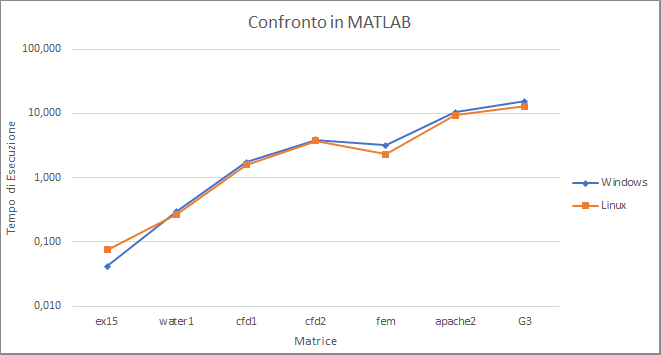
\includegraphics[scale=0.8]{src/plot/TimeMAT.png}
        \caption{Tempi di esecuzione a confronto}
        \label{plot:timemat}
    \end{figure}
    
    \noindent Per quanto riguarda la memoria occupata abbiamo notato, anche in questo caso, come Linux sia in grado di essere migliore di Windows, nonostante si possa notare che per la maggior parte dei casi le differenze sono infinitesimali.\\[0.5cm]
    \begin{figure}[ht]
        \centering
        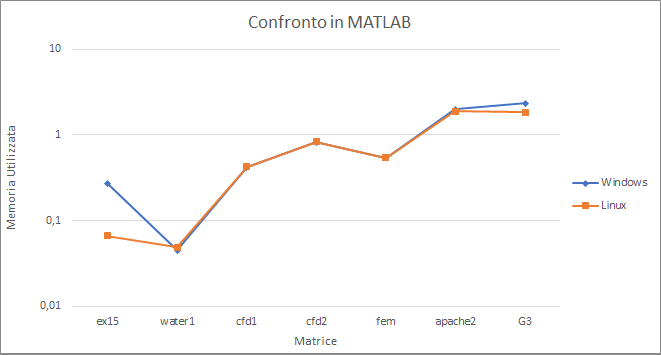
\includegraphics[scale=0.8]{src/plot/MemMAT.png}
        \caption{Memoria occupata a confronto}
        \label{plot:memmat}
    \end{figure}
    
    \newpage
    \noindent Infine come si può notare in figura \ref{plot:memmat} in generale non esistono differenze rilevanti tra i due ambienti.\\[0.5cm]
    \begin{figure}[ht]
        \centering
        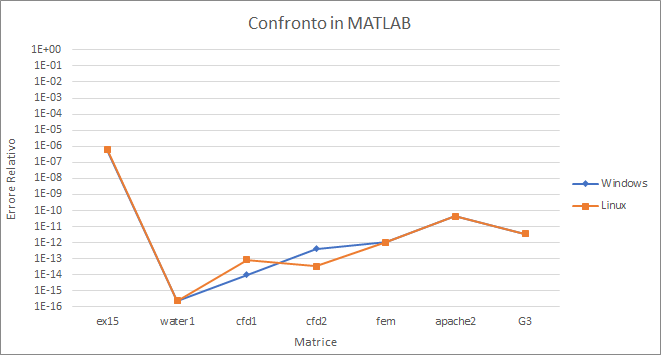
\includegraphics[scale=0.8]{src/plot/ErrMAT.png}
        \caption{Errori Relativi a Confronto}
        \label{plot:errmat}
    \end{figure}
    
    \newpage
    \section{Confronto OCTAVE tra OS}
    \begin{figure}[h]
        \centering
        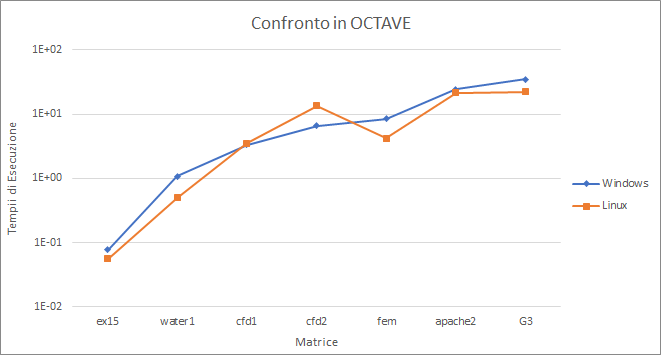
\includegraphics[scale=0.8]{src/plot/TimeOCT.png}
        \caption{Tempi di esecuzione a confronto}
        \label{plot:timeoct}
    \end{figure}
    
    \begin{figure}[h]
        \centering
        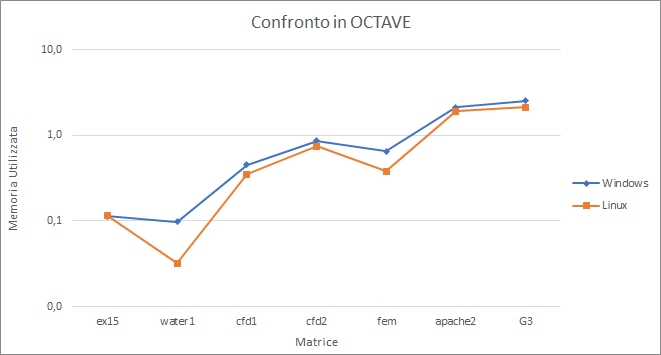
\includegraphics[scale=0.8]{src/plot/MemOCT.png}
        \caption{Memoria occupata a confronto}
        \label{plot:memoct}
    \end{figure}
    
    \begin{figure}[h]
        \centering
        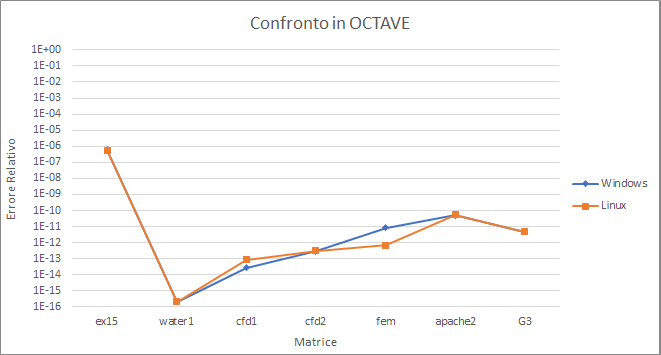
\includegraphics[scale=0.8]{src/plot/ErrOCT.png}
        \caption{Errori Relativi a Confronto}
        \label{plot:erroct}
    \end{figure}
    
    \section{Confronto PYTHON tra OS}
    
    \section{Confronto tra Librerie}
        \subsection{Windows}
        \begin{figure}[h]
            \centering
            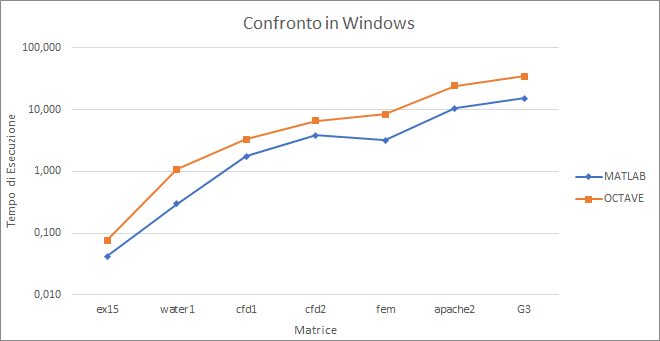
\includegraphics[scale=0.8]{src/plot/WINtime.png}
            \caption{Tempi di esecuzione a confronto}
            \label{plot:timewin}
        \end{figure}
        
        \begin{figure}[h]
            \centering
            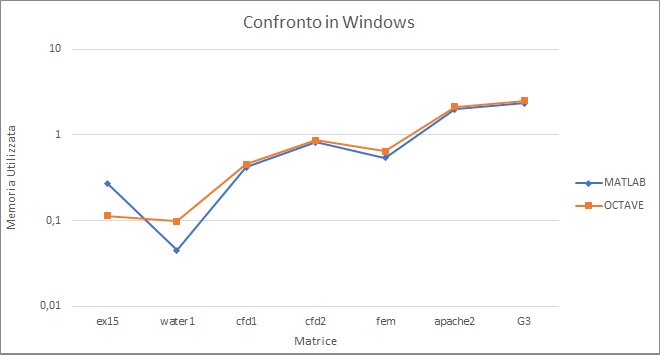
\includegraphics[scale=0.8]{src/plot/WINmem.png}
            \caption{Memoria occupata a confronto}
            \label{plot:memwin}
        \end{figure}
        
        \begin{figure}[h]
            \centering
            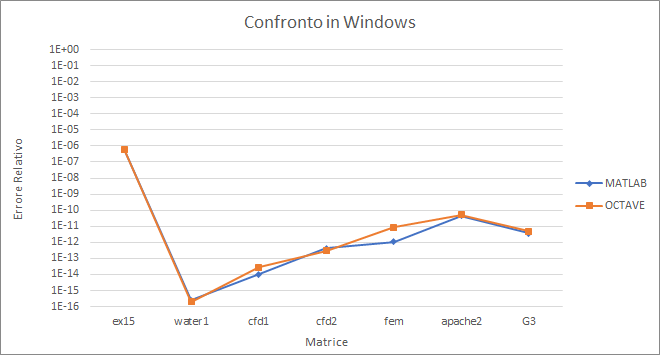
\includegraphics[scale=0.8]{src/plot/WINerr.png}
            \caption{Errori Relativi a Confronto}
            \label{plot:errwin}
        \end{figure}
        
        \subsection{Linux}
        \begin{figure}[h]
            \centering
            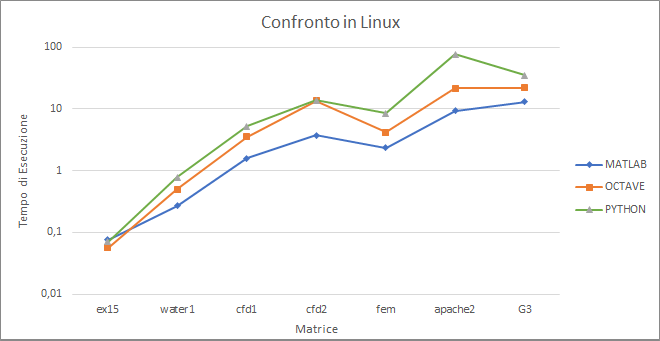
\includegraphics[scale=0.8]{src/plot/LINUXtime.png}
            \caption{Tempi di esecuzione a confronto}
            \label{plot:timelin}
        \end{figure}
        
        \begin{figure}[h]
            \centering
            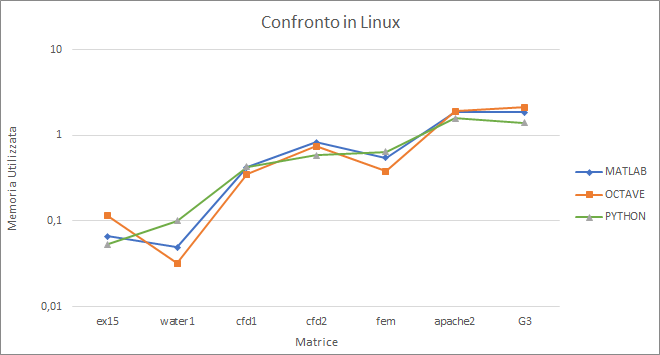
\includegraphics[scale=0.8]{src/plot/LINUXmem.png}
            \caption{Memoria occupata a confronto}
            \label{plot:memlin}
        \end{figure}
        
        \begin{figure}[h]
            \centering
            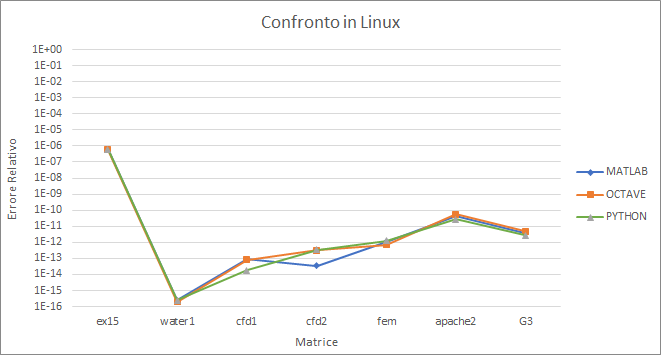
\includegraphics[scale=0.8]{src/plot/LINUXerr.png}
            \caption{Errori Relativi a Confronto}
            \label{plot:errlin}
        \end{figure}

\chapter{Conclusioni}

\nocite{*}
\printbibliography

\end{document}